La figura mostra la gràfica d'una funció $f$. La recta discontínua és una asímptota
vertical; els cercles buits indiquen punts que no pertanyen a la gràfica i els cercles
plens, punts que sí que hi pertanyen.

\begin{center}
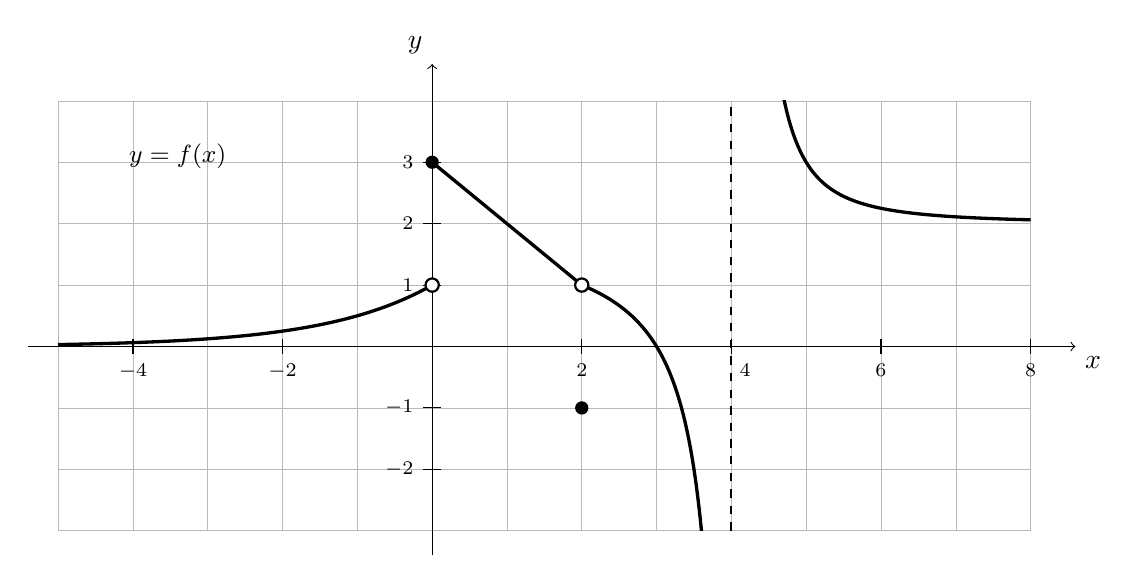
\begin{tikzpicture}[x=0.95cm,y=0.78cm]
  % Branques:  2^x  |  recta (0,3)-(2,1)  |  1-(x-2)/(4-x)  |  2+1/(x-4)^2
  \draw[gray!55,very thin,step=1] (-5,-3) grid (8,4);
  \draw[->] (-5.4,0) -- (8.6,0) node[below right] {$x$};
  \draw[->] (0,-3.4) -- (0,4.6) node[above left] {$y$};
  \foreach \i in {-4,-2,2,6,8} \draw (\i,0.12) -- (\i,-0.12) node[below,font=\scriptsize] {$\i$};
  \draw (4,0.12) -- (4,-0.12) node[below,xshift=5pt,font=\scriptsize] {$4$};
  \foreach \j in {-2,-1,1,2,3} \draw (0.12,\j) -- (-0.12,\j) node[left,font=\scriptsize] {$\j$};
  \draw[dashed,thick] (4,-3) -- (4,4);
  \begin{scope}
    \clip (-5,-3) rectangle (8,4);
    \draw[\colorgrafica,very thick,domain=-5:0,samples=80,smooth] plot (\x,{exp(\x*ln(2))});
    \draw[\colorgrafica,very thick] (0,3) -- (2,1);
    \draw[\colorgrafica,very thick,domain=2:3.7,samples=90,smooth] plot (\x,{1-(\x-2)/(4-\x)});
    \draw[\colorgrafica,very thick,domain=4.35:8,samples=100,smooth] plot (\x,{2+1/((\x-4)^2)});
  \end{scope}
  \draw[fill=white,thick] (0,1) circle (2.4pt);
  \fill (0,3) circle (2.4pt);
  \draw[fill=white,thick] (2,1) circle (2.4pt);
  \fill (2,-1) circle (2.4pt);
  \node[\colorgrafica,font=\small] at (-3.4,3.1) {$y=f(x)$};
\end{tikzpicture}
\end{center}

\begin{apartats}

\apartat[1,25]{0,75}
A partir de la gràfica, determina el valor dels límits següents:
\begin{graella}{4}
  \sa \lim_{x\to-\infty}f(x) & \sa \lim_{x\to0^-}f(x) & \sa \lim_{x\to0^+}f(x) & \sa \lim_{x\to2}f(x)
\end{graella}

\begin{solucio}
i) $0$ \quad ii) $1$ \quad iii) $3$ \quad iv) $1$ (els dos laterals valen $1$).
\end{solucio}

\apartat[1,25]{1}
Estudia la continuïtat de $f$ en $x=0$ i en $x=2$. Si no és contínua, classifica'n la
discontinuïtat i justifica-ho amb el valor de la funció i els límits.

\begin{solucio}
$x=0$: $f(0)=3$ i el lateral dret també val $3$, però l'esquerre val $1$. Laterals finits i
diferents: \textbf{discontinuïtat de salt finit} (de salt $2$).\\
$x=2$: els dos laterals valen $1$, així que $\lim_{x\to2}f(x)=1$, però $f(2)=-1$. El límit
existeix i no coincideix amb la imatge: \textbf{discontinuïtat evitable}.
\end{solucio}

\begin{nomesllarg}
\apartat{0,75}
Estudia què passa en $x=4$ i digues quines asímptotes horitzontals té la gràfica.

\begin{solucio}
En $x=4$, $f(4)$ no existeix i els laterals valen $\lim_{x\to4^-}f(x)=-\infty$ i
$\lim_{x\to4^+}f(x)=+\infty$: \textbf{salt infinit}, amb asímptota vertical $x=4$.\\
Com que $\lim_{x\to-\infty}f(x)=0$ i $\lim_{x\to+\infty}f(x)=2$, hi ha \textbf{dues asímptotes
horitzontals}: $y=0$ per l'esquerra i $y=2$ per la dreta.
\end{solucio}
\end{nomesllarg}

\end{apartats}
